\documentclass{article}
\usepackage{graphicx} % Required for inserting images
\usepackage{amsmath,amssymb,makeidx}

\title{Projet 2 Calcul scientifique numérique}
\author{Mariot Clement et Marchand Leo}
\date{19 novembre 2023}

\begin{document}

\maketitle

\section{Introduction}
    De la même manière que dans le projet précédent, notre but est d'approximer un problème à frontière libre en $C$. En l'occurence, le problème est exactement le même que celui du projet précédent. La
    différence se fait au niveau du calcul de la fonction $f_3$ et nous avons donc étudier l'approximation de l'équation de Fredholm de deuxième espèce. Pour cela, nous avons utilisé deux méthodes d'approximation : la décomposition d'Adomain ainsi que la méthode des noyaux itérés et nous avons comparé les résultats obtenus. Ensuite, il a fallu reprendre le problème afin d'obtenir une nouvelle résolution du problème de Cauchy et enfin reprendre l'algorithme de Newton en l'adaptant à ce nouveau projet.

\section{Méthode de décomposition d'Adomain}
\begin{enumerate}
    \item La première méthode que nous avons implémenté est la méthode de décomposition d'Adomain. Cette méthode revient à approcher la fonction $u$ par : $$u(x)=\sum_{n=0}^{\infty} u_n(x)$$

La suite de fonctions $u_n$ est définie par réccurence :\\

\begin{equation}
    
\left\{
    \begin{array}{ll}
        u_0(x) = f(x) \\
        u_{n+1}(x) = \lambda \displaystyle\int_{a}^{b} k(x,t)u_n(t)dt
    \end{array}
\right.
\end{equation}

Nous allons expliciter la version direct de la suite associée à la méthode de décomposition de adomain :

\begin{equation}
    f_n^\alpha = U_n(x)
\end{equation}
\begin{equation}
    f_n^\alpha = \lambda \displaystyle\int_0^L k(x,s_n)U_{n-1}(s_n) ds_n
\end{equation}
\begin{equation}
    f_n^\alpha = \lambda \displaystyle\int_0^L k(x,s_n) (\lambda\displaystyle\int_0^L k(s_n,s{n-1}) U_{n-2}(s_{n-1})ds_{n-1})ds_n 
\end{equation}
On réarange les intégrales : 
\begin{equation}
    f_n^\alpha = \displaystyle\int_0^L \displaystyle\int_0^L \lambda^2 k(x,s_n)k(s_n,s_{n-1}) U_{n-2}(s_{n-1})ds_n ds_{n-1}
\end{equation}

Par récurrence on obtient :
\begin{equation}
    f_n^\alpha = \displaystyle\int_0^L \ldots \displaystyle\int_0^L \lambda^n k(x,s_n) U_0(s_1)\prod_{i=1}^{n-1} k(s_i, s_{i+1}) ds_1 \ldots ds_n
\end{equation}
En prenant la convention que $s_0 = x$ et $U_0(x) = \frac{h(x)}{\alpha}$ on a :

\begin{equation}
    f_n^\alpha = \displaystyle\int_0^L \ldots \displaystyle\int_0^L \lambda^n \frac{h(s_1)}{\alpha} \prod_{i=1}^n k(s_{i-1},s_i) ds_1 \ldots ds_n
\end{equation}

Donc avec $K(x,s_1,...,s_n)$ une fonction de $h(s_1)$ , de $\prod_{i=1}^n k(s_{i-1},s_i)$  et de $\lambda$ on a donc le résultat:
\begin{equation}
    f_n^\alpha = \displaystyle\int_0^L \ldots \displaystyle\int_0^L K(x,s_1,...,s_n) ds_1 \ldots ds_n
\end{equation}

On a pas utiliser cette méthode de calcul de la suite $(U_n)$ car elle est bien plus compliquée à implementer et nous n'avons pas réussis à la rendre moins coûteuse en temps de calcul que la définition par récurrence. Ainsi par la suite on utilisera un calcul par récurrence de la suite pour la méthode de décompisition de Adomain.


On a donc eu à programmer cette méthode pour approximer $f_3$. Nous allons donc par la suite détailler le code établi.

\item A l'aide de l'expression précédente, on peut trouver une nouvelle expression de

\item Pour ce code, nous avons repris quelques fonctions du projet précédent : 
- la solution exacte :

{
\includegraphics[width=10cm]{solex.jpg} \par}
\bigskip

- la fonction d'approximation d'intégrale de Gauss Legendre que nous avons adaptée pour fonctionner avec un vecteur de cinq points en entrée :\\

{
\includegraphics[width=14cm]{gauss.jpg} \par}
\bigskip

- la définition des fonctions $k$ et $h$ utile pour le calcul de $f_3$ :\\

{
\includegraphics[width=10cm]{k.jpg} \par}
\bigskip

{
\includegraphics[width=10cm]{h.jpg} \par}
\bigskip

On a ensuite pu définir la fonction Adomain qui est donc notre nouvel outil d'approximation de $f_3$ :\\

{
\includegraphics[width=10cm]{adomain1.jpg} \par}
\bigskip

{
\includegraphics[width=10cm]{adomain2.jpg} \par}
\bigskip

{
\includegraphics[width=10cm]{adomain3.jpg} \par}
\bigskip

\item Enfin, pour valider la méthode, nous l'avons utilisée pour approcher une fonction dont on connaît la valeur exacte de l'intégrale. Nous avons pris l'exemple du poly page $10$ qui est : $u(x)=e^x-x+x\displaystyle\int^1_0tu(t)dt$. On devait alors trouver comme approximation $u(x)=e^x$. Voici ce que l'on obtient:
{
\includegraphics[width=10cm]{comparaison_méthodes_test.png} \par}
\bigskip

\item On remarque que la méthode de décomposition de Adomain approche le comportement de la solution exacte mais la méthode des noyaux itérés ne semble pas convenir pour $x$ lorsque ce dernier n'est pas dans le voisinage de $1$. Ces erreurs peuvent avoir plusieurs origines telles qu'un bug dans le code ou alors le fait que l'on itère seulement vingt fois, etc...

\end{enumerate}


\section{Méthode des noyaux itérés}

\begin{enumerate}
    \item La méthode des noyaux itérés est semblable à la méthode précédente. La différence se fait sur la création de la suite. En effet, il n'est plus question d'utiliser la série des $u_n$ pour trouver la fonction recherchée. La fonction va ici être approché par la limite de la suite lorsque $n\longrightarrow +\infty$. Il y'a donc un changement dans l'expression de la suite des $u_n$ qui devient :\\
    $$u_{n+1}(x)=f(x) + \lambda \displaystyle\int_{a}^{b} k(x,t)u_n(t)dt$$ 

    On prendra $u_o(x)=f(x)$ comme pour la méthode d'Adomain.

    \item Voici donc le code utilisé pour la méthode; ce code est très similaire à celui de la méthode d'Adomain.\\

    {
\includegraphics[width=14cm]{noyaux1.jpg} \par}
\bigskip

{
\includegraphics[width=10cm]{noyaux2.jpg} \par}
\bigskip



    {
\includegraphics[width=8cm]{noyaux3.jpg} \par}
\bigskip

    \item Enfin, de même que pour Adomain, nous avons tester cette méthode sur un cas simple où la solution exacte est facile à calculer. Nous sommes alors tomber sur un résultat similaire.


\end{enumerate}


\section{Résolution du problème de Cauchy}
    

    Dans cette partie, nous avons repris la structure du code du projet précédent en modifiant juste l'approximation de $f_3$ avec les deux nouvelles méthodes. Nous allons donc comparer les différentes erreurs obtenues avec les deux méthodes ainsi que la valeur du $\alpha$ optimal.

\bigskip

    - \textbf{Pour la méthode d'Adomain} :

     On commence par la recherche du $\alpha$ optimal. On obtient ainsi la courbe suivante :

     
     \bigskip
    {
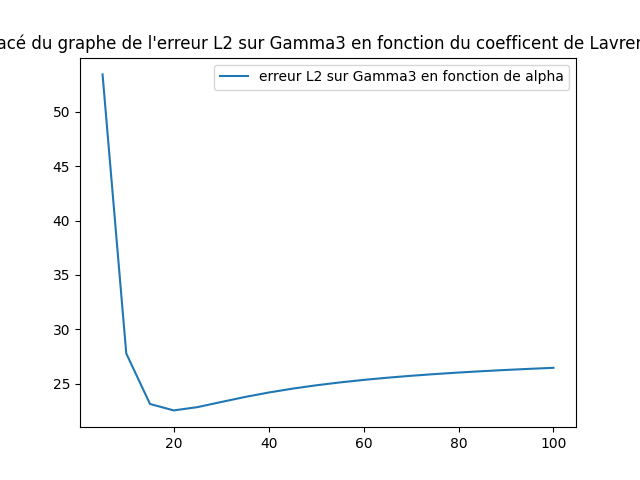
\includegraphics[width=10cm]{Etude_erreur_selon_alpha_adomain.png} \par}
\bigskip

    On en déduit ainsi empiriquement que $\alpha = 20$ et c'est celui que l'on utilisera par la suite pour la méthode de décomposition de Adomain.

    \bigskip

    On trace la solution exacte sur $\Omega$ :

        {
    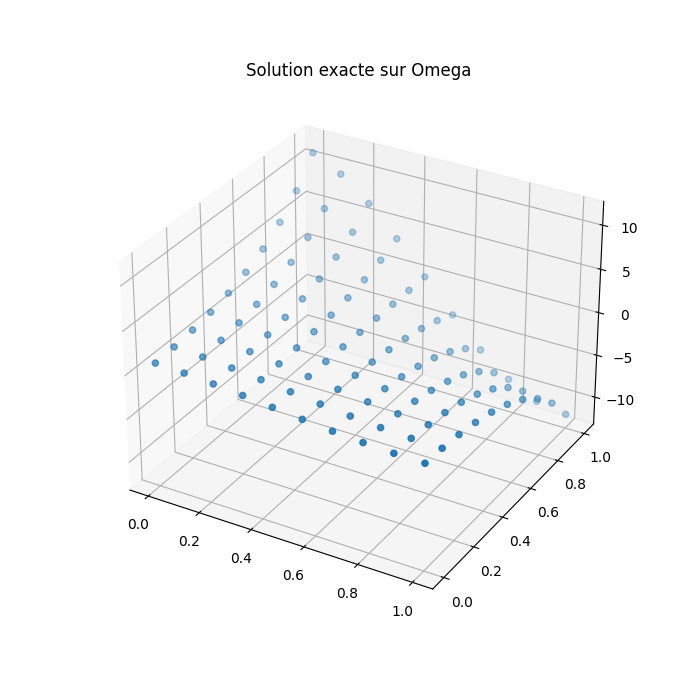
\includegraphics[width=9cm]{solex_omega.png} \par}
    \bigskip
     Puis la solution approchée par la méthode de décomposition de Adomain :

    {
    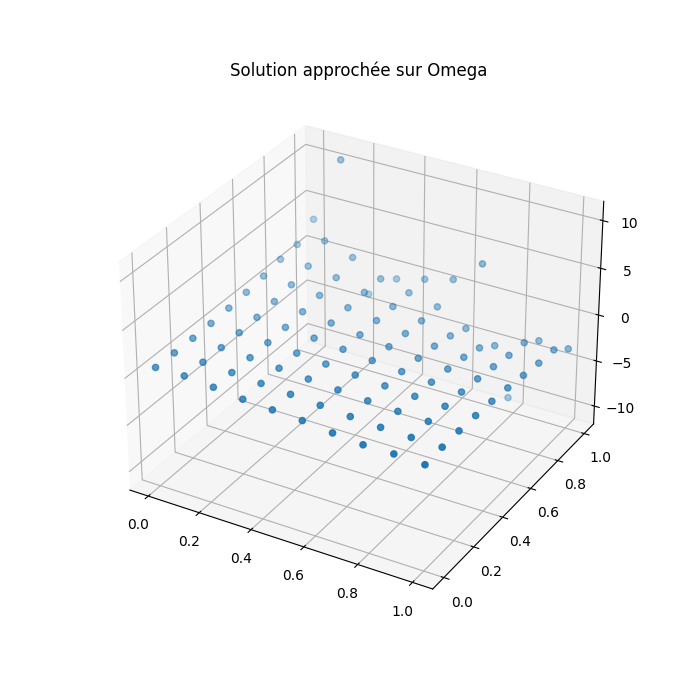
\includegraphics[width=9cm]{calc_adomain.png} \par}
    \bigskip

    Et enfin la différence entre la solution approchée et exacte :

    {
    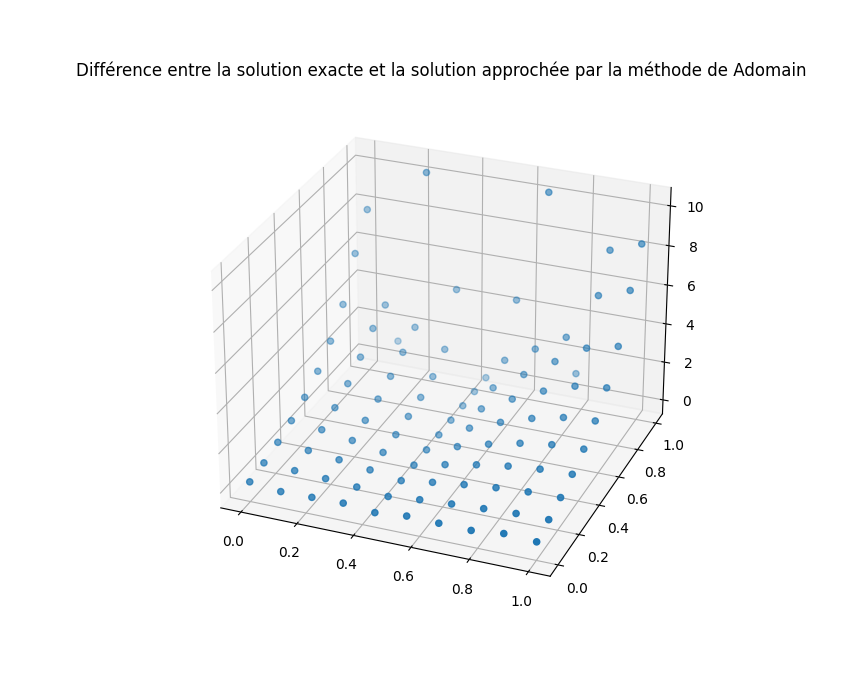
\includegraphics[width=9cm]{Diff_adomain.png}\par}
    \bigskip

    On remarque ainsi que la grande partie de l'erreur commise par la solution approchée est au voisinage de $\Gamma_3$. Cela nous indique potentiellement une mauvaise approximation de la fonction $f_3$ qui est la condition sur ce bord. Maintenant, regardons si la méthode des noyaux itérés donne de meilleures approximations.
    
    
    \bigskip
    
    
    - \textbf{Pour la méthode des noyaux itérés} :

    
    On recommence par une recherche du $\alpha$ optimal pour cette nouvelle méthode de résolution de l'intégrale de seconde espèce de Fredholm régularisée, ainsi on obtient :

    {
    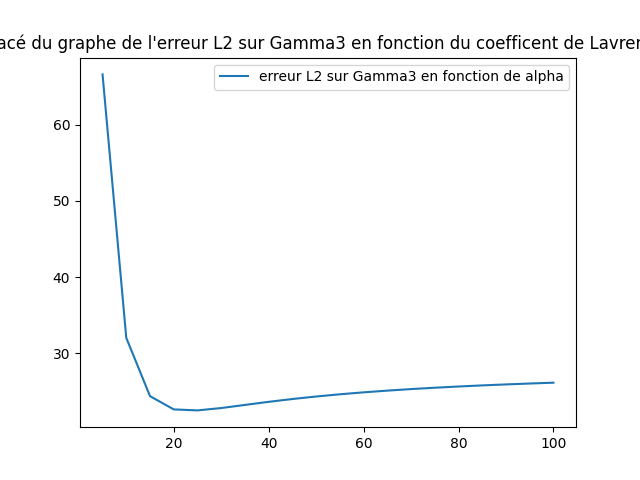
\includegraphics[width=9cm]{Etude_erreur_selon_alpha_noyaux.png} \par}
    \bigskip
    Cela mène à choisir $\alpha = 21 $ comme optimum. On trace maintenant la solution approchée par la méthode des noyaux itérés sur $\Omega$ :

    {
    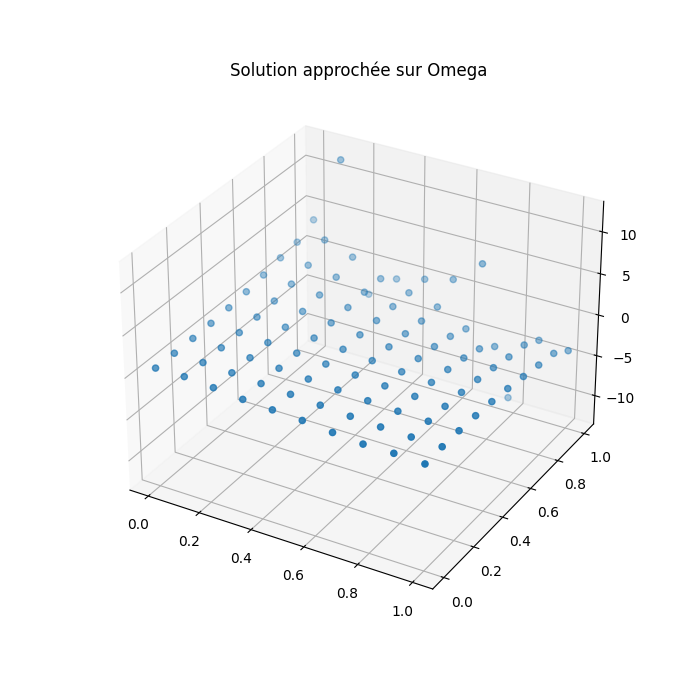
\includegraphics[width=9cm]{calc_noyaux.png} \par}
    \bigskip

    Enfin voici la différence entre la solution exacte et la solution approchée par la méthode des noyaux itérés:

    {
    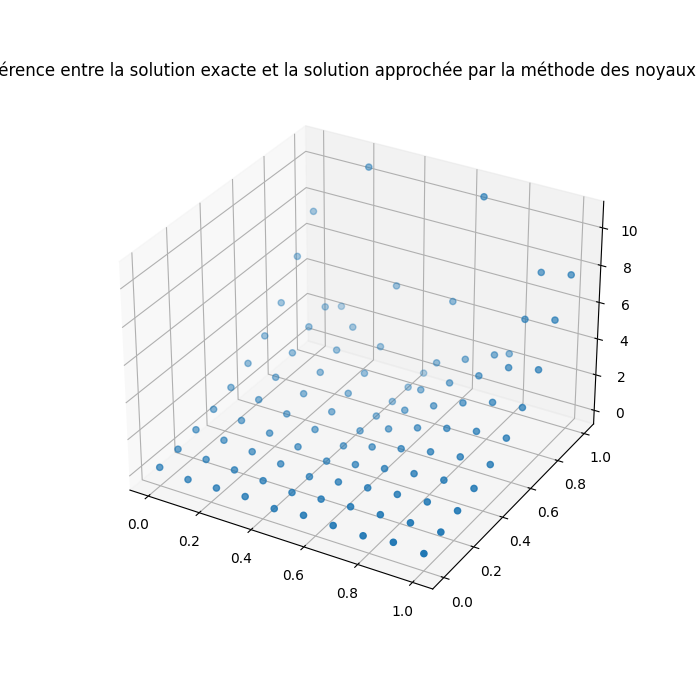
\includegraphics[width=9cm]{Diff_noyaux.png} \par}
    \bigskip

    On remarque que l'erreur commise en chaque point du maillage est sensiblement la même que pour la méthode de décomosition de Adomain ce qui révèlerait que la résolution du problème de cauchy n'est pas valide ou bien le code contient encore quelques bugs.
    
\section{Algorithme de Newton}

    De même que dans la section précédente, nous avons repris le programme du projet précédent pour réaliser la recherche de la forma de la frontière à l'aide de l'algorithme de Newton. Ce dernier est donc codé comme celà :\\

    {
\includegraphics[width=10cm]{newton.jpg} \par}
\bigskip
On rappelle que la frontière ne peut être trouvée en $x=0.5$ car il n'y a pas unicité de la solution car la solution exacte donne $u_{ex}(0.5,y) = 0$, $\forall  y \in [0;H]$.
On recherche maintenant une frontière constante d'équation $y = 0.5$. Ce qui nous donne pour la méthode de décompostion de Adomain :


    {
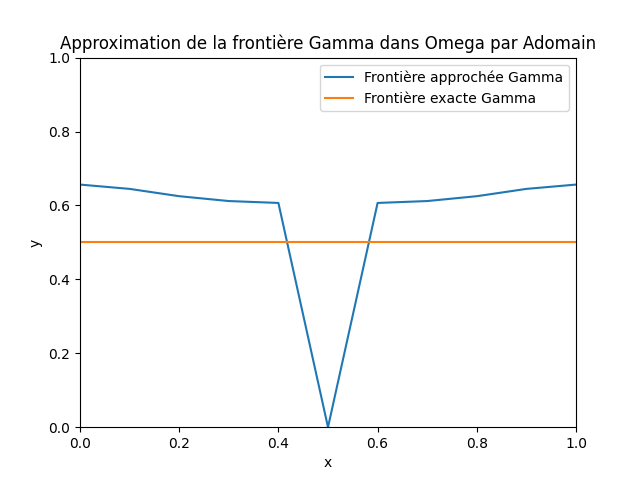
\includegraphics[width=10cm]{frontiere_constante_adomain.png} \par}
\bigskip

Et de la même manière pour la méthode des noyaux itérés :

    {
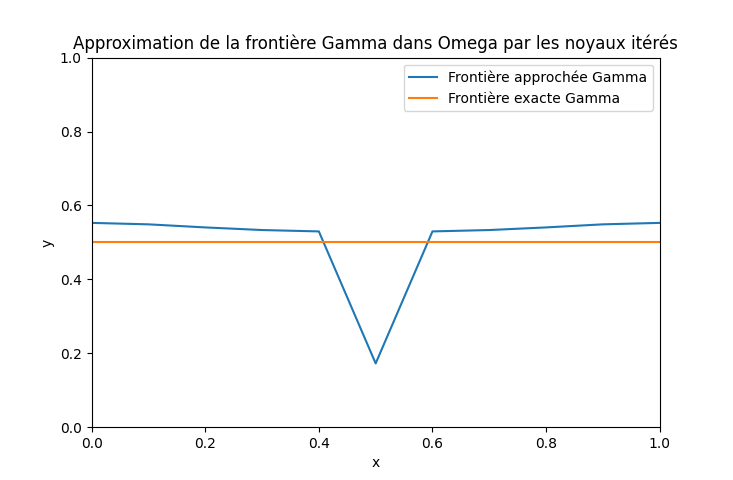
\includegraphics[width=10cm]{frontiere_constante_noyaux.png} \par}
\bigskip

Pour la recherche de cette forme de frontière la méthode des noyaux itérés semble donner de meilleurs resultats même si les deux méthodes capturent le comportement global de la frontière exacte.

Regardons ce que la méthode de décomposition de Adomain donne pour une frontière d'équation $y = 03.x + 0.3$:

    {
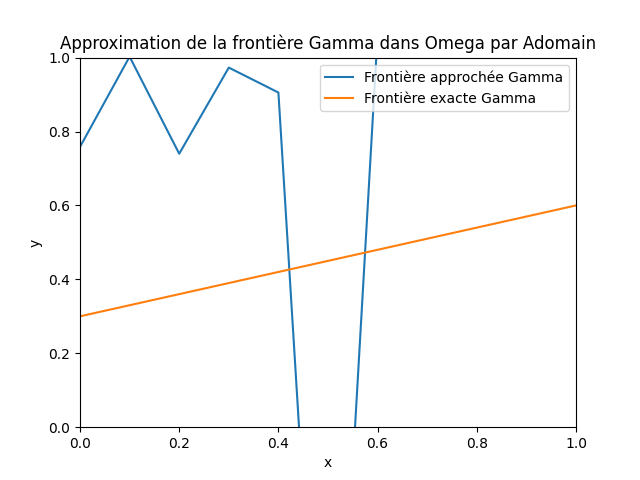
\includegraphics[width=10cm]{frontiere_affine_adomain.png} \par}
\bigskip

On a ici un soucis probablement causé par la mauvaise qualité de l'approximation car l'algorithme de Newton a été testé et est normalement performante.

    {
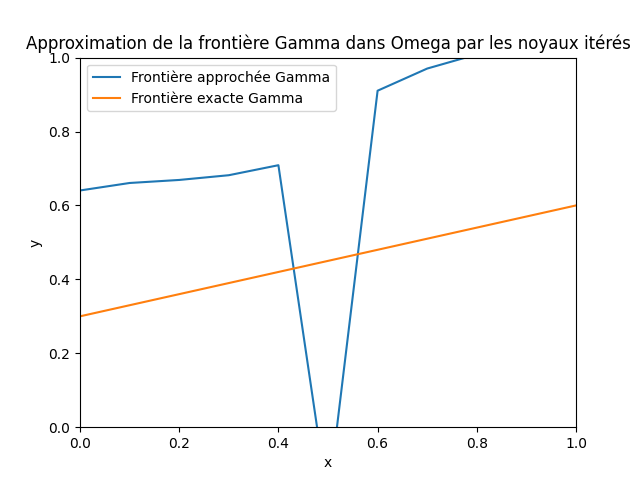
\includegraphics[width=10cm]{frontiere_affine_noyaux.png} \par}
\bigskip

On a le même problème dans ce cas ci mais cette méthode semble capturer légèrement le comportement de la frontière pour des $x$ assez petits.

Enfin maintenant on regarde ce que l'on obtient pour une frontière d'équation $y = 0.5sin(\pi x) + 0.2$ pour la méthode de décomposition de Adomain:

    {
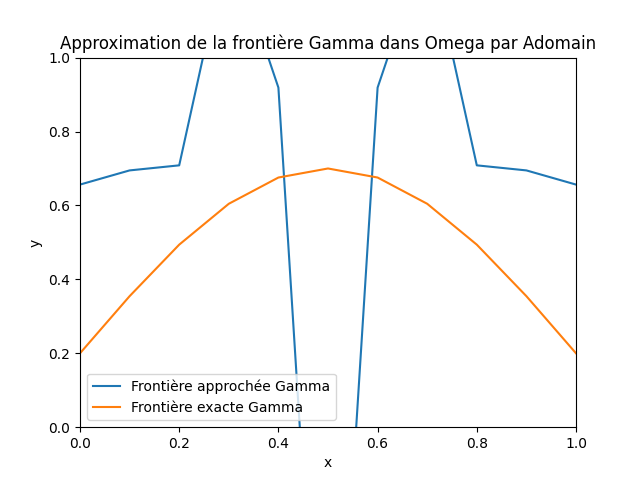
\includegraphics[width=10cm]{frontiere_sinus_adomain.png} \par}
\bigskip

La méthode des noyaux itérés nous donne :

    {
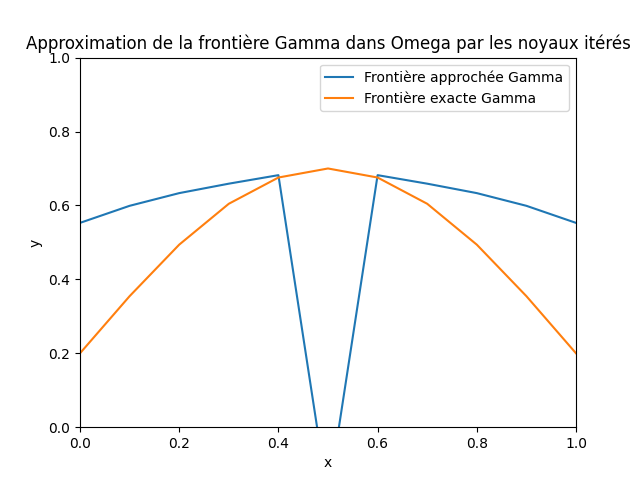
\includegraphics[width=10cm]{frontiere_sinus_noyaux.png} \par}
\bigskip

Encore une fois la méthode des noyaux itérés donne une meilleure approximation de la frontière $\Gamma_3$.

\section{Conclusion}
Pour conclure cette comparaison entre la méthode de décomposition de Adomain et la méthode des noyaux itérés, on remarque que la méthode des noyaux itérés donne de meilleures approximations de frontières de diverses formes. D'un point de vue technique les deux méthodes ont les mêmes difficultées d'implémentation, c'est-à-dire d'itéré les quadratures sur $u_n(x)$ pour obtenir une somme d'itérés ou bien la limite de la suite $(u_n)$. Ainsi nous préconisons l'utilisation de la méthode des noyaux itérés.

\end{document}
